\documentclass{beamer}

\usepackage[utf8]{inputenc}
\usepackage{adjustbox}
\usepackage{setspace}
\usepackage{amsmath}
\usepackage{amsthm}
\usepackage{amssymb}
\usepackage{xcolor}
\usepackage{listings}
\usepackage{pgfplots}

\definecolor{codegreen}{rgb}{0,0.6,0}
\definecolor{codegray}{rgb}{0.5,0.5,0.5}
\definecolor{codepurple}{rgb}{0.58,0,0.82}
\definecolor{backcolour}{rgb}{0.95,0.95,0.92}
 
\lstdefinestyle{mystyle}{
    backgroundcolor=\color{backcolour},   
    commentstyle=\color{codegreen},
    keywordstyle=\color{magenta},
    numberstyle=\tiny\color{codegray},
    stringstyle=\color{codepurple},
    basicstyle=\footnotesize,
    breakatwhitespace=false,         
    breaklines=true,                 
    captionpos=b,                    
    keepspaces=true,                 
    numbers=none,                    
    numbersep=5pt,                  
    showspaces=false,                
    showstringspaces=false,
    showtabs=false,                  
    tabsize=2
}
 
\lstset{style=mystyle}
\lstset{language=Python}

\usetheme{Berlin}
\setbeamertemplate{mini frames}{} 
\usecolortheme{default}

\title{Pynqrypt}
\author{Roberto Alessandro Bertolini}
\institute{FPGA101 - Politecnico di Milano}
\date{\today}
\subtitle{A FPGA-accelerated encryption library for PYNQ}

\makeatletter
\setbeamertemplate{headline}{%
	\begin{beamercolorbox}[colsep=1.5pt]{upper separation line head}
	\end{beamercolorbox}
	\begin{beamercolorbox}{section in head/foot}
		\vskip2pt\insertsectionnavigationhorizontal{\paperwidth}{}{}\vskip2pt
	\end{beamercolorbox}%
	\ifbeamer@theme@subsection%
	%\begin{beamercolorbox}[colsep=1.5pt]{middle separation line head}
	%\end{beamercolorbox}
	%\begin{beamercolorbox}[ht=2.5ex,dp=1.125ex,%
	%	leftskip=.3cm,rightskip=.3cm plus1fil]{subsection in head/foot}
	%	\usebeamerfont{subsection in head/foot}\insertsubsectionhead
	%\end{beamercolorbox}%
	\fi%
	\begin{beamercolorbox}[colsep=1.5pt]{lower separation line head}
	\end{beamercolorbox}
}
\makeatother

\setbeamertemplate{caption}{\raggedright\insertcaption\par}

\begin{document}

\begin{frame}
    \titlepage
\end{frame}

\section{Introduction}

\subsection{AES}
\begin{frame}
    \frametitle{Encryption Algorithms}

    \begin{block}{AES}
    \onslide<2->AES is a symmetric-key algorithm for secure encryption and decryption. It is widely used in both industry and government to protect sensitive data.
    \end{block}

    \onslide<3->\begin{block}{AES-CTR}
    \onslide<4->AES-CTR is a mode of operation for the AES block cipher. It is a highly-parallelizable and efficient encryption algorithm, well suited for hardware acceleration.
    \end{block}
\end{frame}

\subsection{Software Performance}
\begin{frame}
    \frametitle{Performance Considerations}

    Security usually comes at the cost of performance.
    \onslide<2->High performance systems have no trouble satisfying these requirements, but the same cannot be said for low-power embedded systems.

    \onslide<3->\begin{adjustbox}{max height=2in, center}
        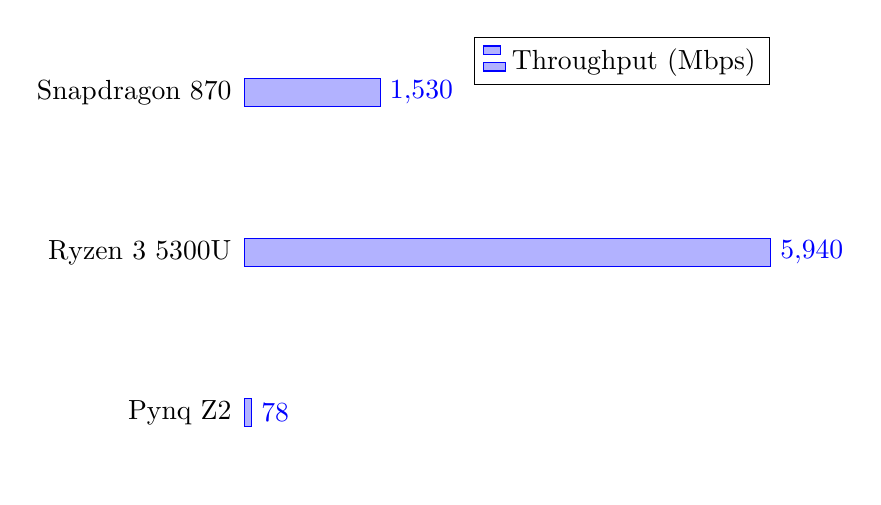
\begin{tikzpicture}
            \begin{axis}[
                    xbar,
                    y axis line style = { opacity = 0 },
                    axis x line       = none,
                    tickwidth         = 0pt,
                    enlarge y limits  = 0.2,
                    enlarge x limits  = 0.02,
                    symbolic y coords = {Pynq Z2, Ryzen 3 5300U, Snapdragon 870},
                    ytick=data,
                    nodes near coords,
                ]
                \addplot coordinates { (78,Pynq Z2) (5940,Ryzen 3 5300U) (1530,Snapdragon 870) };
                \legend{Throughput (Mbps)}
            \end{axis}
        \end{tikzpicture}
    \end{adjustbox}
\end{frame}

\section{Pynqrypt}

\subsection{Introduction}
\begin{frame}
    \frametitle{What is Pynqrypt}

    Pynqrypt is a Python library for data encryption with the AES-CTR algorithm.
    \begin{itemize}
        \onslide<2->\item Works on every platform supported by PYNQ (with the appropriate bitstream)
        \onslide<3->\item Compatible with other AES-CTR implementations
        \onslide<4->\item Fast
    \end{itemize}
\end{frame}

\subsection{Performance}
\begin{frame}
    \frametitle{Performance Comparison}

    \onslide<2->\begin{adjustbox}{max height=3in, center}
        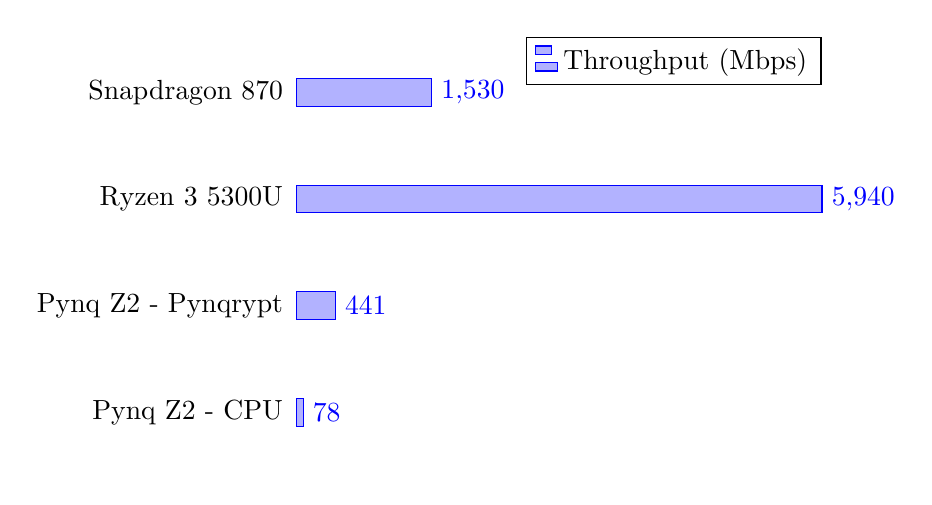
\begin{tikzpicture}
            \begin{axis}[
                    xbar,
                    y axis line style = { opacity = 0 },
                    axis x line       = none,
                    tickwidth         = 0pt,
                    enlarge y limits  = 0.2,
                    enlarge x limits  = 0.02,
                    symbolic y coords = {Pynq Z2 - CPU, Pynq Z2 - Pynqrypt, Ryzen 3 5300U, Snapdragon 870},
                    ytick=data,
                    nodes near coords,
                ]
                \addplot coordinates { (78,Pynq Z2 - CPU) (441,Pynq Z2 - Pynqrypt) (5940,Ryzen 3 5300U) (1530,Snapdragon 870) };
                \legend{Throughput (Mbps)}
            \end{axis}
        \end{tikzpicture}
    \end{adjustbox}
\end{frame}

\subsection{Usage}
\begin{frame}[fragile]
    \frametitle{Usage}

    \onslide<2->\begin{lstlisting}
    from pynqrypt import Pynqrypt
    import numpy as np
    \end{lstlisting}

    \onslide<3->\begin{lstlisting}
    pynqrypt = Pynqrypt(file='./bistream.xsa', post_ap=True)
    \end{lstlisting}

    \onslide<4->\begin{lstlisting}
    data = np.frombuffer(..., np.uint8)

    pynqrypt.set_key(...)
    pynqrypt.set_nonce(...)
    pynqrypt.set_length(len(data))
    \end{lstlisting}
\end{frame}

\begin{frame}[fragile]
    \frametitle{Usage}

    \onslide<2->\begin{lstlisting}
    input_buffer = pynqrypt.get_input_array()
    output_buffer = pynqrypt.get_output_array()

    input_buffer[:] = data[:]

    pynqrypt.prepare()
    pynqrypt.run_blocking()
    \end{lstlisting}

    \onslide<3->\begin{lstlisting}
    output_buffer.invalidate()

    ... = bytes(output_buffer)

    pynqrypt.cleanup()
    \end{lstlisting}
\end{frame}

\section{Demo}

\subsection{Demo Time}
\begin{frame}
    \frametitle{USBCrypt: let's see it in action!}
\end{frame}

\section{Conclusion}

\subsection{Issues}
\begin{frame}
    \frametitle{Issues Encountered}

    \begin{itemize}
        \onslide<2-> \item Issue: Vitis HLS doesn't work\\Solution: install Ubuntu 22.04 LTS
        \onslide<3-> \item Issue: Vitis HLS doesn't work\\Solution: install \texttt{libncurses5-dev}
        \onslide<4-> \item Issue: Vitis HLS doesn't work\\Solution: install \texttt{g++} and other buildtools
        \onslide<5-> \item Issue: Vitis HLS doesn't work\\Solution: always do a clean build of the project
        \onslide<6-> \item Issue: my IP doesn't work\\Solution: wire all the ports\\\onslide<7-> Maybe rewatch the lesson? 
    \end{itemize}
\end{frame}

\subsection{Project Takeaways}
\begin{frame}
    \frametitle{Conclusions}

    \begin{block}{Advantages}
        \begin{itemize}
            \onslide<2-> \item Low-power systems can greatly benefit from offloading intensive tasks to an FPGA accelerator
            \onslide<3-> \item On-the-fly reconfigurability allows for multiple libraries to share the same hardware
        \end{itemize}
    \end{block}

   \onslide<4->\begin{alertblock}{Drawbacks}
        \begin{itemize}
            \onslide<5-> \item Not every task is suitable for an FPGA, and some platform-specific optimization is required for best results
            \onslide<6-> \item Hardware accelerated libraries might not always be a drop-in replacement, some code refactoring might be required
        \end{itemize}
   \end{alertblock}
\end{frame}

\begin{frame}
    \frametitle{Personal Thoughts}

    \begin{itemize}
        \onslide<2-> \item Vitis HLS is magical, and makes it easy to write software for FPGAs...\\\onslide<3->... but it is also broken, badly documented and finicky to use.
        \onslide<4-> \item Pynq is a great platform for development and prototyping, but it is not intuitive to use and the documentation is lacking.
        \onslide<5-> \item Sometimes I felt like I was just throwing things at the wall and hoping they would stick.
    \end{itemize}
\end{frame}

\subsection{End}
\begin{frame}
    \frametitle{The End}

    \large Thanks for your attention!
\end{frame}

\end{document}
